\subsection{Use cases}\label{ssc:usecases}
Below, the following use cases have been derived from the understanding of the problem domain and actors described in the previous sections. The following description of the use cases include how the interactions with the system will take place, which actors are involved, and which functions are called, within the system to complete the actions.
\par
in addition to the already described interactions, the system definition has stated, based on the interviews with Aalborg Zoo, that the admin should be able to print out a report of assets from the system. The report will consist of a number of assets and take shape as a file, saved on the admins computer.
\par
Each use case has been described and is followed by a diagram of the interaction.
\newline

\fancyLayout{use_case}{Add an asset}
    {Use case for adding an asset}
    {use_case:add_an_asset}
    {
        \textbf{Use Case:} Adding an asset is done by the admin. An admin goes to the add asset page, attaches the relevant tags, and fills in the relevant information about the asset. The admin then saves the asset in the system and it becomes visible to all employees.
    
        \vskip 0.2cm
        
        \textbf{Objects:} Admin, Asset
        
        \vskip 0.2cm
        
        \textbf{Functions:} Add asset
    }

\begin{figure}[H]
    \centering
    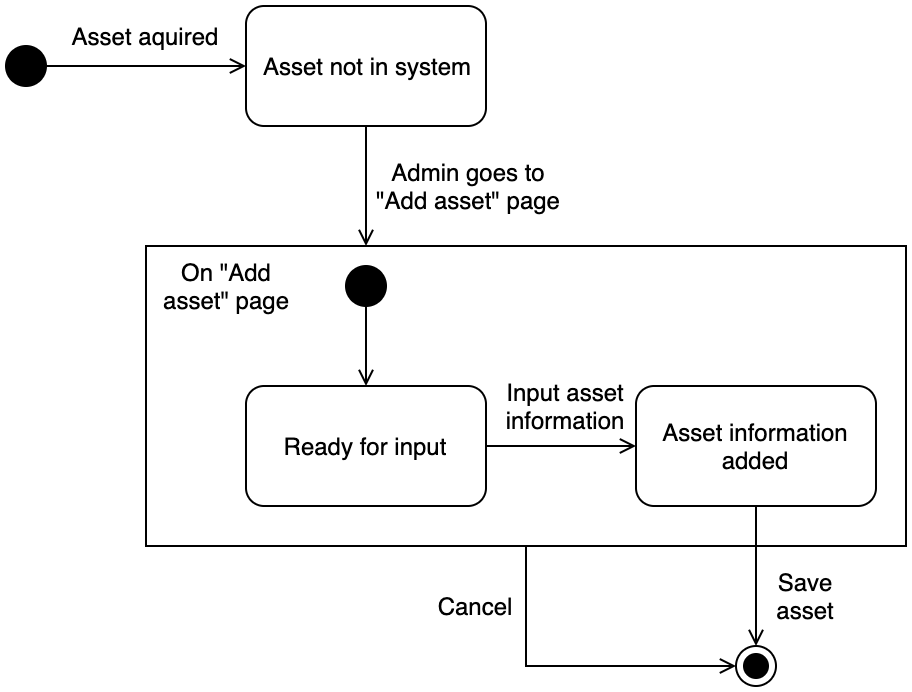
\includegraphics[width=0.8\textwidth]{figures/UseCases/UC_Add_asset.png}
    \caption{User interface state chart diagram for adding an asset}
    \label{fig:add_asset_statechart}
\end{figure}

\newpage

\fancyLayout{use_case}{Loan out an asset}
    {Use case for loaning out an asset}
    {use_case:loan_out_an_asset}
    {
        \textbf{Use Case:} Loaning out an asset is being carried out by an admin, whom an employee contacts, when they want to borrow the given asset. The admin goes to the page of the given asset and attaches the employees tag to it. The admin then hands over the asset to the employee.
    
        \vskip 0.2cm
        
        \textbf{Objects:} Admin, Asset, Employee, Tag
        
        \vskip 0.2cm
        
        \textbf{Functions:} Asset loaned out, Tag attached to asset
    }
 
\begin{figure}[H]
    \centering
    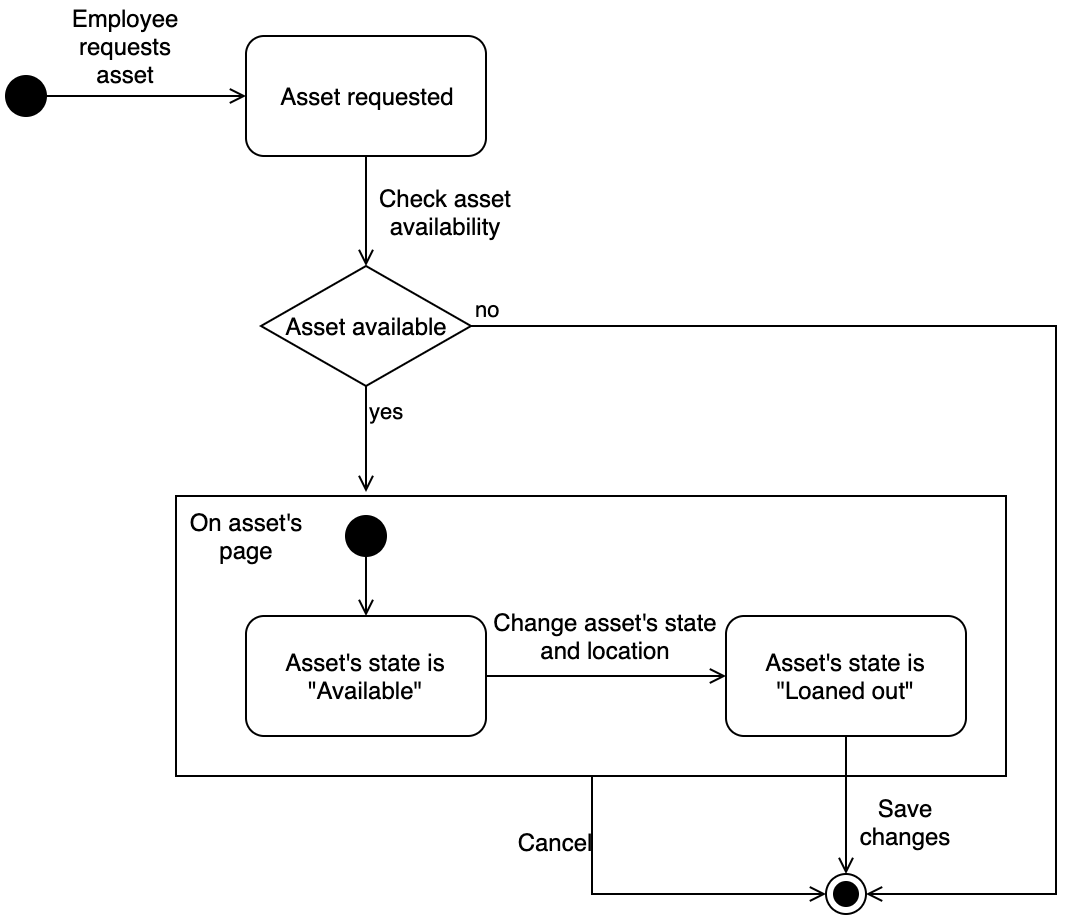
\includegraphics[width=0.8\textwidth]{figures/UseCases/UC_Loan_out_asset.png}
    \caption{User interface state chart diagram for loaning out an asset}
    \label{fig:loan_out_asse_statechart}
\end{figure}
\todo{Update diagram}
 
\fancyLayout{use_case}{Return an asset}
    {Use case for returning an asset}
    {use_case:return_an_asset}
    {
        \textbf{Use Case:} When an asset is being returned by an employee, it is handed over to an admin. The admin then goes to the page of the given asset and detaches the tag of the given employee from the asset.
    
        \vskip 0.2cm
        
        \textbf{Objects:} Admin, Asset, Employee, Tag
        
        \vskip 0.2cm
        
        \textbf{Functions:} Update asset information, Tag detached from asset
    }
    
\begin{figure}[H]
    \centering
    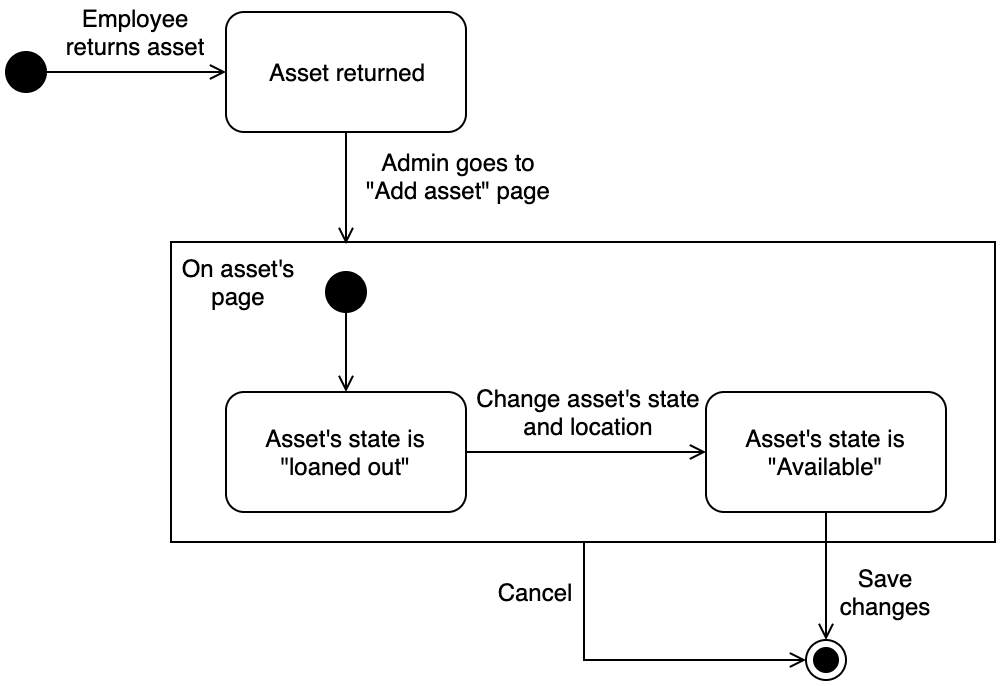
\includegraphics[width=0.8\textwidth]{figures/UseCases/UC_Return_asset.png}
    \caption{User interface state chart diagram for returning an asset}
    \label{fig:return_asset_statechart}
\end{figure}
\todo{Update diagram}

\fancyLayout{use_case}{Change the information of an asset}
    {Use case for changing the information of an asset}
    {use_case:changing_the_information_about_an_asset}
    {
        \textbf{Use Case:} If one of the states of an asset changes, these changes should be updated in the system by an admin. These state changes could be things such as the asset going from working to being broken, or being updated to a new operation system. To update the asset's information, the admin goes to the given asset's page, potentially through the search page. The admin can then press the edit button and change the outdated data to comply to the new state of the asset in the problem domain.
    
        \vskip 0.2cm
        
        \textbf{Objects:} Admin, Asset
        
        \vskip 0.2cm
        
        \textbf{Functions:} Search for asset, Update asset information, View asset
    }
    
\begin{figure}[H]
    \centering
    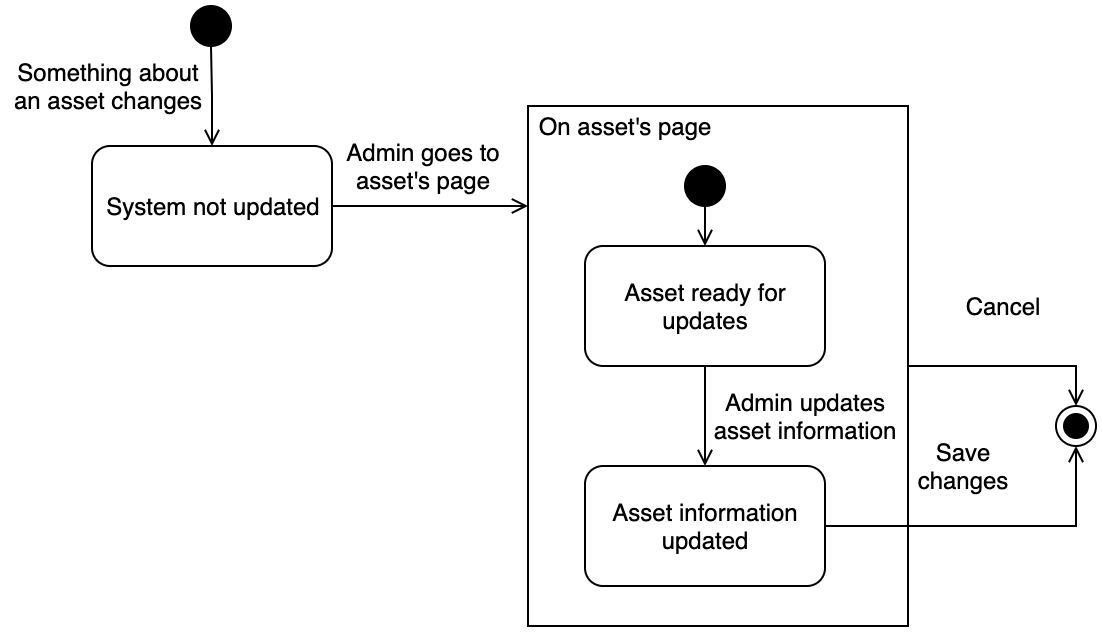
\includegraphics[width=0.8\textwidth]{figures/UseCases/UC_Change_asset.png}
    \caption{User interface state chart diagram for changing an asset}
    \label{fig:edit_asset_statechart}
\end{figure}

\newpage

\fancyLayout{use_case}{Remove an asset}
    {Use case for removing an asset}
    {use_case:remove_an_asset}
    {
        \textbf{Use Case:} When an asset is no longer needed within the problem domain, it is discarded. This is handled in the system by an admin. The admin goes to the page of the given asset and deletes it from the system. The asset is then removed from the system and is no longer visible to any of the employees.
    
        \vskip 0.2cm
        
        \textbf{Objects:} Admin, Asset, Employee
        
        \vskip 0.2cm
        
        \textbf{Functions:} Remove asset
    }

\begin{figure}[H]
    \centering
    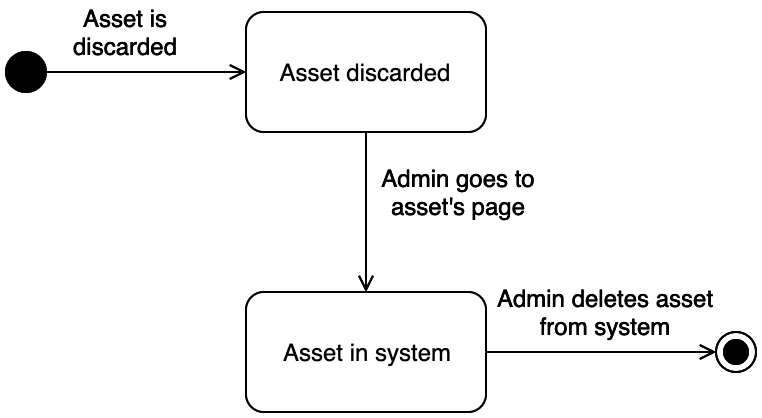
\includegraphics[width=0.8\textwidth]{figures/UseCases/UC_Remove_asset.png}
    \caption{User interface state chart diagram for removing an asset}
    \label{fig:remove_asset_statechart}
\end{figure}

\newpage

\fancyLayout{use_case}{Search for an asset}
    {Use case for searching for an asset}
    {use_case:search_for_an_asset}
    {
        \textbf{Use Case:} If an employee needs to know something about an asset or an admin needs to see a specific asset, this can be achieved by going to the search page, choosing a department, and entering some information about the asset in the search field. The system then returns a list of assets complying with the search query. The employee can then chose an asset and go to its page.
    
        \vskip 0.2cm
        
        \textbf{Objects:} Admin, Asset, Employee
        
        \vskip 0.2cm
        
        \textbf{Functions:} Search for asset, View asset
    }

\begin{figure}[H]
    \centering
    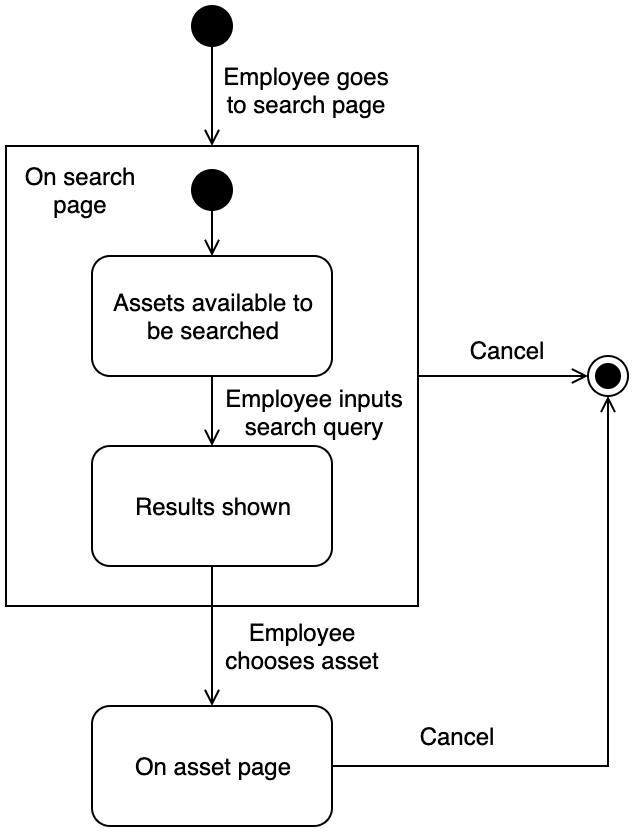
\includegraphics[width=0.6\textwidth]{figures/UseCases/UC_Search_asset.png}
    \caption{User interface state chart diagram for searching for an asset}
    \label{fig:search_asset_statechart}
\end{figure}

\fancyLayout{use_case}{Print a report of assets}
    {Use case for printing a report of assets}
    {use_case:print_a_report_of_assets}
    {
        \textbf{Use Case:} As the number of assets increases in the system, an admin might want to retrieve a number of assets to see outside of the system. The admin goes to the search page and enters a search query, which the assets they want to retrieve from the system must comply with. The admin then selects a number of assets and presses the print button. The system then generates a file containing information about the selected assets and saves it on the admins computer.
    
        \vskip 0.2cm
        
        \textbf{Objects:} Admin, Asset
        
        \vskip 0.2cm
        
        \textbf{Functions:} Export report, Search of asset
    }

\begin{figure}[H]
    \centering
    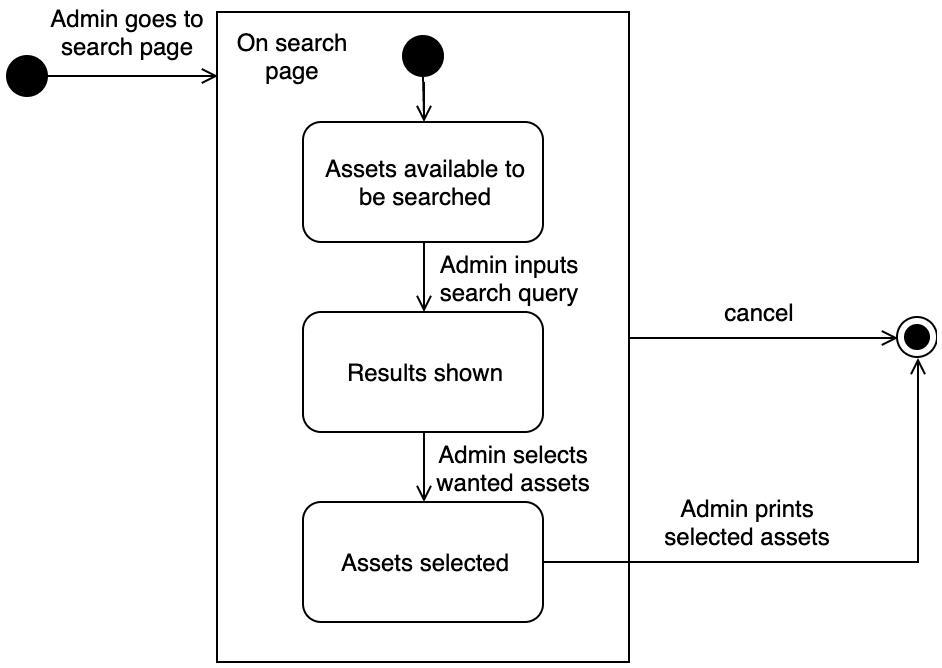
\includegraphics[width=0.8\textwidth]{figures/UseCases/UC_Print_report.png}
    \caption{User interface state chart diagram for printing out a report}
    \label{fig:print_report_statechart}
\end{figure}

\fancyLayout{use_case}{Comment an asset}
    {Use case for commenting on an asset}
    {use_case:commenting_on_an_asset}
    {
        \textbf{Use Case:} An employee might have a comment regarding an asset they have borrowed, such as an issue they had with it or suggestions for improvements. To make an admin aware of this, they can go to the page of the asset and add a comment to it. This comment will be visible to all admin.
    
        \vskip 0.2cm
        
        \textbf{Objects:} Admin, Asset, Employee
        
        \vskip 0.2cm
        
        \textbf{Functions:} Add comment to asset, Search for asset, View Asset
    }

\begin{figure}[H]
    \centering
    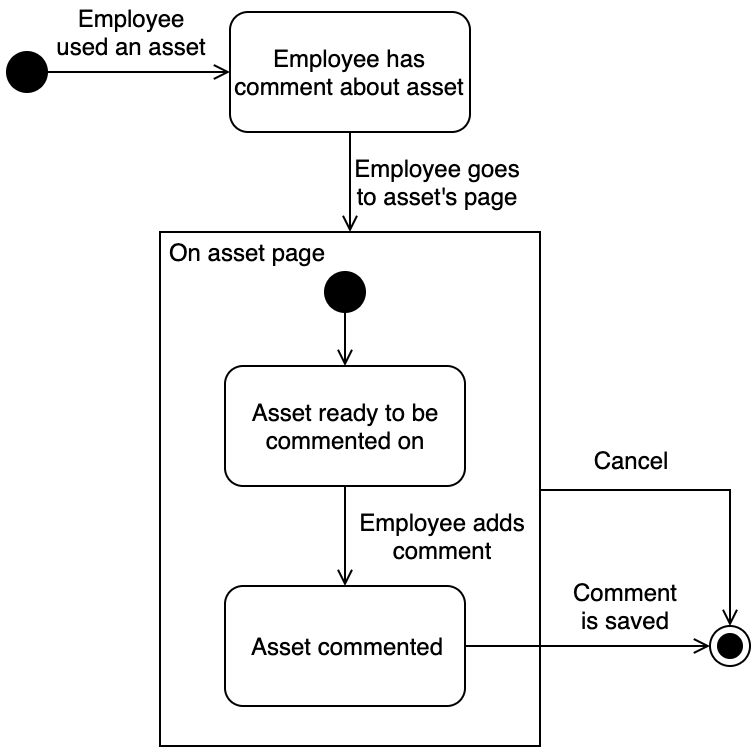
\includegraphics[width=0.8\textwidth]{figures/UseCases/UC_Add_comment.png}
    \caption{User interface state chart diagram for adding a comment to an asset}
    \label{fig:add_comment_statechart}
\end{figure}

These are the relevant use cases to handle the assets, and they have been placed in an actor table with the twp previously mentioned actors, to illustrate the connections between these.

\begin{table}[H]
    \centering
    % \hrule
    \vspace{0.2cm}
    \hspace{6cm} \vspace{0.6cm} \textbf{Actors}
    \begin{tabular}{p{0.5\textwidth} || p{0.2\textwidth} p{0.2\textwidth}}
        \textbf{Use cases} & Admin & Employee \vspace{0.2cm}\\
        \hline \hline
        Add an asset & \hspace{0.34cm} \checkmark & \\
        \hline
        Loan out an asset & \hspace{0.34cm} \checkmark & \hspace{0.6cm} \checkmark \\
        \hline
        Return an asset & \hspace{0.34cm} \checkmark & \hspace{0.6cm} \checkmark \\
        \hline
        Change the information about an asset & \hspace{0.34cm} \checkmark & \\
        \hline
        Remove an asset & \hspace{0.34cm} \checkmark & \\
        \hline
        Search for an asset & \hspace{0.34cm} \checkmark & \hspace{0.6cm} \checkmark \\
        \hline
        Print a report of assets & \hspace{0.34cm} \checkmark & \\
        \hline
        Comment an asset & & \hspace{0.6cm} \checkmark\\
    \end{tabular}
    \vspace{0.2cm}
    % \hrule
    \vspace{0.2cm}
    \caption{Actor table of the relations between actors and use cases.}
    \label{tab:actor_table}
\end{table}

In the actor table above has shown that the admin takes part in almost every use case. This can be explained by the way the system will be used. The system should function almost like an interface to a database, so it makes sense that the admin will be involved in all the changes made to the system and, as an effect of this, the database.
\par

The defined use cases have then been used to extract relevant functions and, later in the report, construct the user interface. For most of these use cases, the system should limited the access of employee without the admin atatus, which has resulted in two more functions, \textit{Authenticate user} and \textit{Check access level}. These functions are used to garantee that parts of the system is only accessible to employees with admin status and are executed on login and most of the described use cases above.\\

The functions discovered in this section have been analysed and described in the following section.